%%%%%%%%%%%%%%%%%%%%%%% file template.tex %%%%%%%%%%%%%%%%%%%%%%%%%
%
% This is a template file for Web of Conferences Journal
%
% Copy it to a new file with a new name and use it as the basis
% for your article
%
%%%%%%%%%%%%%%%%%%%%%%%%%% EDP Science %%%%%%%%%%%%%%%%%%%%%%%%%%%%
%
%%%\documentclass[option comma separated list]{webofc}
%%%Three important options:
%%% "epj" for EPJ Web of Conferences Journal
%%% "bio" for BIO Web of Conferences Journal
%%% "mat" for MATEC Web of Conferences Journal
%%% "itm" for ITM Web of Conferences Journal
%%% "e3s" for E3S Web of Conferences Journal
%%% "shs" for SHS Web of Conferences Journal
%%% "twocolumn" for typesetting an article in two columns format (default one column)
%
\documentclass{webofc}
\usepackage[varg]{txfonts}   % Web of Conferences font
\usepackage{listings}
\usepackage{hyperref}
\usepackage{amsmath}
\lstset
{
    language=[LaTeX]TeX,
    breaklines=true,
    basicstyle=\tt\small
}
%
% Put here some packages required or/and some personnal commands

\newcommand{\todo}[1]{{\bf #1}}
\newcommand{\bigO}{\mathcal{O}}
\newcommand{\savg}[1]{\left<#1\right>}
\newcommand{\svar}{{\rm Var}}
\newcommand{\scov}{{\rm Cov}}
\newcommand{\Mshft}{\mathbf{M}_{\theta_2}}
\newcommand{\dMshft}{\partial\Mshft}
\newcommand{\dA}{\partial A}
\newcommand{\dB}{\partial B}
\newcommand\numberthis{\addtocounter{equation}{1}\tag{\theequation}}
%
%
\begin{document}

%
\title{A fast template periodogram}
%
% subtitle is optionnal
%
%%%\subtitle{Do you have a subtitle?\\ If so, write it here}


\author{\firstname{John} \lastname{Hoffman}\inst{1}\fnsep\thanks{\href{mailto:jah5@princeton.edu}{\tt jah5@princeton.edu}} \and
        \firstname{Jake} \lastname{VanderPlas}\inst{2}\fnsep\thanks{\href{mailto:jakevdp@cs.washington.edu}{\tt jakevdp@cs.washington.edu}} \and
        \firstname{Joel} \lastname{Hartman}\inst{1}\fnsep\thanks{\href{mailto:jhartman@astro.princeton.edu}{\tt jhartman@astro.princeton.edu}} \and
        \firstname{G\'asp\'ar} \lastname{Bakos}\inst{1}\fnsep\thanks{\href{mailto:gbakos@astro.princeton.edu}{\tt gbakos@astro.princeton.edu}} 
        % etc.
}
\institute{Department of Astrophysical Sciences, Princeton University, Princeton NJ 08540 \and
           eScience Institute, University of Washington, Seattle, WA 98195
}
\abstract{%
  This proceedings presents a novel, non-linear extension to the Lomb-Scargle periodogram that allows periodograms to be generated
  for arbitrary signal shapes. Such periodograms are already known as "template periodograms" or "periodic matched filters," but 
  current implementations are computationally inefficient. The "fast template periodogram" presented here improves existing techniques
  by a factor of $\sim$a few for small test cases ($\bigO(10)$ observations), and over three orders of magnitude for lightcurves containing
  $\bigO(10^4)$ observations. The fast template periodogram scales asymptotically as $\bigO(HN_f\log HN_f + H^4N_f)$, where
  $H$ denotes the number of harmonics required to adequately approximate the template and $N_f$ is the number of trial
  frequencies. Existing implementations scale as $\bigO(N_{\rm obs}N_f)$, where $N_{\rm obs}$ is the number of
  observations in the lightcurve. An open source Python implementation is available on GitHub.
}
%
\maketitle
%


\section{Introduction}\label{sec:intro}
Template fitting, or periodic matched filtering, is a powerful technique for identifying, classifying, and characterizing
periodic variability in noisy time series data. However, template fitting requires several orders of magnitude more computational
resources than running a Lomb Scargle periodogram \cite{Lomb_1976,Scargle_1982,Barning_1963,Vanicek_1971} on the same lightcurve, 
and the computational requirements scale as $N_{\rm obs}N_f$, where $N_{\rm obs}$ is the number of observations in the 
lightcurve and $N_f$ is the number of trial frequencies.

For example, \cite{Sesar_etal_2016} used template fitting to model RR Lyrae in the Pan-STARRS DR1 \cite{PanSTARRS} and found that, 
for a given completeness, template fitting produced purer samples of RR Lyrae than Lomb-Scargle or multi-term extensions \cite{Palmer_2009}.
However, \cite{Sesar_etal_2016} found that the computational resources needed to produce template fits 
(approximately 30 minutes per source per CPU), limited the number of lightcurves for which a full template fit could be 
performed to $\bigO(10^3)$ out of $\bigO(10^6)$ Pan-STARRS DR1 lightcurves.

Pan-STARRS lightcurves typically have less than 35 observations in 5 photometric filters ($\sim7$ per filter), but many photometric surveys 
have orders of magnitude more observations --- CoRoT \cite{CoRoT}, SuperWASP \cite{SuperWASP}, HATNet \cite{HATNet}, 
and Kepler \cite{Kepler}, for example, have $\bigO(10^4-10^5)$ observations per lightcurve. Since template fitting scales as 
$\bigO(N_{\rm obs}^2),$\footnote{The actual scaling is technically $\bigO(N_{\rm obs}N_f)$, 
however the number of trial frequencies $N_f$ scales linearly with $N_{\rm obs}$ 
\cite{Vanderplas+Ivezic_2015}.} running template periodograms on these surveys currently requires a prohibitively 
large amount of computational resources. 

However, if template periodograms were computationally efficient enough to run on entire surveys with $\bigO(10^3-10^5)$ observations
per lightcurve, they have the potential to be a powerful tool for automated classification. For example, by selecting a group of templates
that capture the variety of periodic signals present in astrophysical data, a template periodogram could provide \emph{simultaneous} detection
and (pre-)classification of all lightcurves with higher signal to noise than multi-harmonic periodograms, which are also designed to 
detect non-sinusoidal signals. 

The advantage of templates is that there are only three free parameters (amplitude, phase, and a constant offset),
compared to the multi-harmonic periodogram, which has $2H+1$ free parameters, where $H$ is the number of harmonics. Using a collection
of templates encodes ``domain knowledge'' \cite[see, e.g.][]{Yu+Simoff+Jan_2010} into the periodogram, which helps to reduce the parameter space 
to a set of physically plausible lightcurve shapes. 

\section{Extending Lomb-Scargle to arbitrary shapes}\label{sec:formulation}

The Lomb-Scargle periodogram \cite{Lomb_1976,Scargle_1982,Barning_1963,Vanicek_1971} is also known as least squares spectral analysis. 
The formulation of the periodogram given in \cite{Lomb_1976} and \cite{Scargle_1982} fits a linear model

\begin{equation}\label{eq:lsmodel}
\hat{y}(t|\theta, \omega) = \theta_1\cos{\omega t} + \theta_2\cos{\omega t}
\end{equation}

\noindent to time series data $D = \{t_n, y_n, \sigma_n|n < N\}$ at a number of trial frequencies $\omega$. The Lomb-Scargle periodogram,

\begin{equation}\label{eq:ls}
    P_{\rm LS}(\omega) = \frac{1}{2\sigma^2}\left(\frac{\left[\sum_{n=1}^N (y_n - \bar{y})\cos{\omega t_n}\right]^2}{\sum_{n=1}^N \cos^2{\omega t_i}} + \frac{\left[\sum_{n=1}^N (y_n - \bar{y})\sin{\omega t_n}\right]^2}{\sum_{n=1}^N \sin^2{\omega t_i}} \right),
\end{equation}

\noindent is similar to a Fourier intensity for unevenly spaced data. As shown in \cite{Scargle_1982}, the periodogram can be derived by minimizing the squared residuals and setting

\begin{equation}\label{eq:chi2pdg}
P(\omega) = \frac{\chi^2_0 - \chi^2(\omega)}{\chi^2_0},
\end{equation}

\noindent where $\chi^2(\omega)$ is the minimum (weighted) sum of squared residuals for a model fit at frequency $\omega$, and $\chi^2_0$ is the
weighted sum of squared residuals for a constant fit.

There are many extensions to the Lomb-Scargle periodogram that are useful for time domain astronomy. \cite{Zechmeister+Kurster_2009} 
used \emph{weighted} squared residuals and added a constant offset to $\hat{y}$, \cite{Schwarzenberg-Czerny_1996,Palmer_2009} further extended the Lomb-Scargle 
periodogram for models with more than one harmonic

\begin{equation}\label{eq:lsharm}
\hat{y}(t|\theta, \omega) = \theta_0 + \sum_{h=1}^{H}\theta_{2h}\cos{h\omega t} + \theta_{2h - 1}\sin{h\omega t},
\end{equation}

\noindent and recently \cite{Vanderplas+Ivezic_2015} provided a formalism for applying periodograms to multi-band time series.

The multiharmonic periodogram is designed to find non-sinusoidal periodic signals in irregularly spaced time series data. However,
as shown in \cite{Vanderplas+Ivezic_2015}, increased flexibility comes at a cost -- the noise level of the periodogram relative to the 
maximum peak height tends to increase as the number of free parameters in the model $\hat{y}$ increases, and in some cases the best frequency
can tend to a harmonic or a subharmonic of the true frequency.

If the signal shape of interest is known \emph{a priori} and can be expressed as a truncated Fourier series with 
$H$ harmonics 

\begin{equation}\label{eq:template}
M(\omega t) = \sum_{h=1}^{H}\psi_{2h}\cos{h \omega t} + \psi_{2h-1}\sin{h \omega t},
\end{equation}

\noindent then a model of the form

\begin{equation}\label{eq:yhatftp}
\hat{y}_M(t|\theta, \omega) = \theta_0 + \theta_1 M(\omega (t - \theta_2))
\end{equation}

\noindent should provide improved signal to noise over the multiharmonic periodogram, since there are only three free parameters at
each trial frequency, regardless of the number of harmonics used to express the template $M$. The difference between the template
periodogram (i.e., the periodogram derived from $\hat{y}_M$) and the multiharmonic periodogram of \cite{Schwarzenberg-Czerny_1996,Palmer_2009} is that the
harmonic amplitudes $\psi_i$ are \emph{not free parameters} in the template periodogram, while they are free parameters for the 
multiharmonic periodogram.

Unlike the Lomb-Scargle extensions previously mentioned, the template periodogram is \emph{non-linear}. The non-linearity arises
from the phase shift parameter $\theta_2$. For Lomb-Scargle and multiharmonic periodograms, the phase shift is equivalent
to changing the relative amplitudes of the cosine and sine terms. This is not true for the template periodogram, since $\psi_i$ terms
are deliberately fixed. Instead, by working with $x \equiv \cos{\omega \theta_2}$, the template can be expressed as:

%\begin{equation}\label{eq:mshift}
\begin{align*}
M(\omega (t - \theta_2)) &= \sum_{h=1}^H \left[\left(\psi_{2h}T_h(x) \mp \psi_{2h-1}\sqrt{1 - x^2}U_{h-1}(x)\right)\cos{h\omega t} \right.\\
&\quad\quad \left.+ \left(\psi_{2h-1}T_h(x) \pm \psi_{2h}\sqrt{1 - x^2}U_{h-1}(x)\right)\sin{h\omega t}\right]\numberthis \label{eq:mshift}
\end{align*}
%\end{equation}

\noindent where $T_n$ and $U_n$ are the Chebyshev polynomials of the first and second kind, respectively, and the $\pm$ sign ambiguity
reflects the two possible signs of $\sin{\omega\theta_2}$. 

Detailed derivations of the template periodogram will be presented in a later paper, but the non-linearity of the template periodogram
can be reduced to finding the real roots of a polynomial of order $\sim 6H$ at each trial frequency. The root finding step 
scales as $\bigO(H^3-H^4)$ at each trial frequency, and the polynomial coefficients can be computed with a single non-equispaced 
fast fourier transform (NFFT \cite{NFFT}) of size $N_fH$. Thus, the template periodogram scales as 

\begin{equation}\label{eq:scaling}
\bigO( N_fH^4 + N_f H\log N_f H ).
\end{equation}


\section{Implementation}\label{sec:implementation}
A Python implementation of the fast template periodogram is available at 
\begin{center}
\href{https://github.com/PrincetonUniversity/FastTemplatePeriodogram}{\tt https://github.com/PrincetonUniversity/FastTemplatePeriodogram}. 
\end{center}

\begin{figure}
\centering

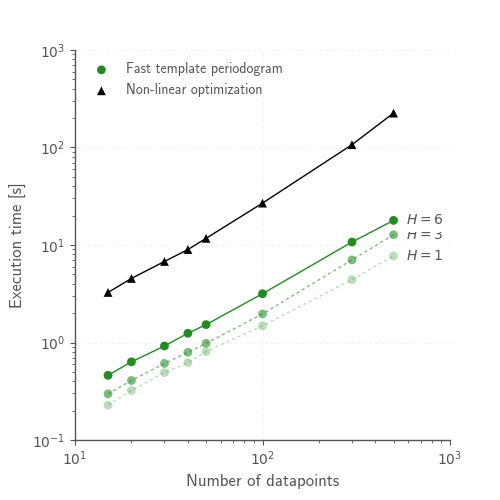
\includegraphics[width=6cm,clip]{../plots/timing_vs_ndata.png}
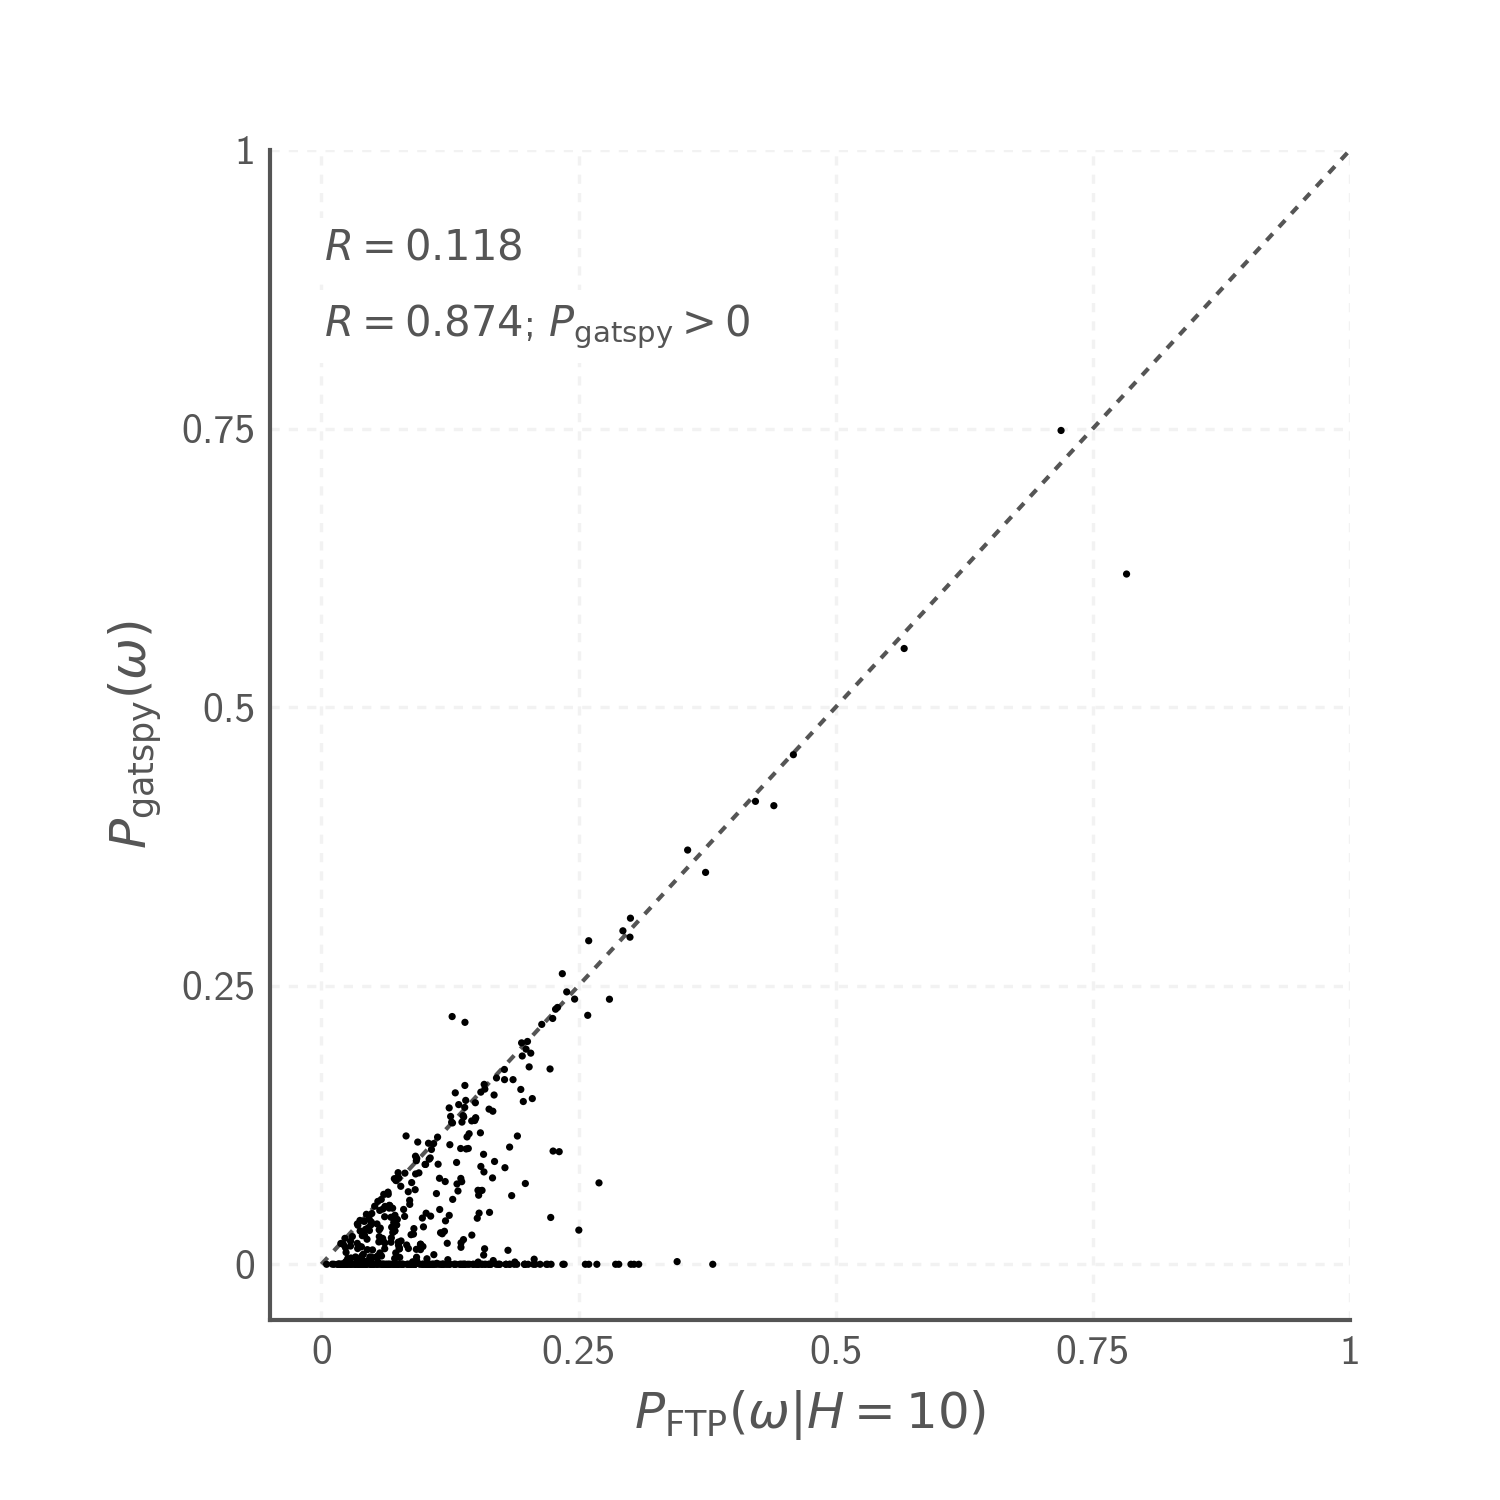
\includegraphics[width=6cm,clip]{../plots/correlation_with_gatspy.png}
\caption{Timing (\emph{left}) and accuracy (\emph{right}) comparisons between the \texttt{gatspy} \cite{gatspy} template fitting algorithm 
and the fast template periodogram. The fast template periodogram improves computational efficiency by a factor of $\sim$a few for small test cases
and this improvement factor grows linearly in $\bigO(N_f\sim N_{\rm obs})$. Though the fast template periodogram has $\bigO(N_f\log N_f)$ asymptotic scaling for a given value of $H$, the root-finding utilities (which scale as $\bigO(N_f)$) dominate the computational time for all test cases shown here. In most cases, the fast template periodogram finds better template fits than \texttt{gatspy} (points that fall below the dashed line on the \emph{right}-most figure).}
\label{fig:timingacc}
\end{figure}

Timing comparisons with an existing Python template fitting implementation (\texttt{gatspy} \cite{gatspy}) shown in Figure \ref{fig:timingacc}
demonstrate the improved computational efficiency of the fast template periodogram. In terms of accuracy, Figure \ref{fig:timingacc} also
shows that the fast template periodogram, which solves for the optimal parameters directly, is usually able to find better
fits than the \texttt{gatspy} implementation, which uses non-linear optimization tools to find the optimal parameters. 

\section{Conclusion}\label{sec:conclusion}

Finding non-sinusoidal signals in irregularly spaced astrophysical data is a challenging problem that requires balancing model flexibility
against the need to use as few model parameters as possible to minimize the relative noise of the periodogram. Template periodograms,
or periodic matched filters, allow for the detection of periodic signals with fixed, arbitrary non-sinusoidal shapes without the increase
of periodogram noise inherent in the multiharmonic periodogram presented in \cite{Schwarzenberg-Czerny_1996,Palmer_2009}. However,
template periodogram implementations to date \cite{Sesar_etal_2016,gatspy} have relied on non-linear optimization at each trial frequency
to obtain the optimal amplitude, phase, and offset of the template. Thus, applying template periodograms to large photometric surveys
like Pan-STARRS \cite{PanSTARRS} require prohibitive amounts of computational resources and scale as $\bigO(N_fN_{\rm obs}\sim N_{\rm obs}^2)$.

However, template periodograms can be made orders of magnitude more computationally efficient. By using the algorithmic shortcuts described here,
template periodograms could potentially prove computationally feasible on large photometric surveys with many ($\gtrsim 10^2$) observations per 
lightcurve, like CoRoT \cite{CoRoT}, HATNet \cite{HATNet}, and others. An open source implementation of the fast template periodogram is 
available on GitHub, and improvements to the existing implementation should continue to improve computational efficiency. 


\bibliography{procrefs}
\end{document}

% end of file template.tex

